\section{Appendix}
\subsection{Baseline and Optimized Query Comparison}

\begin{figure*}[t]
\centering
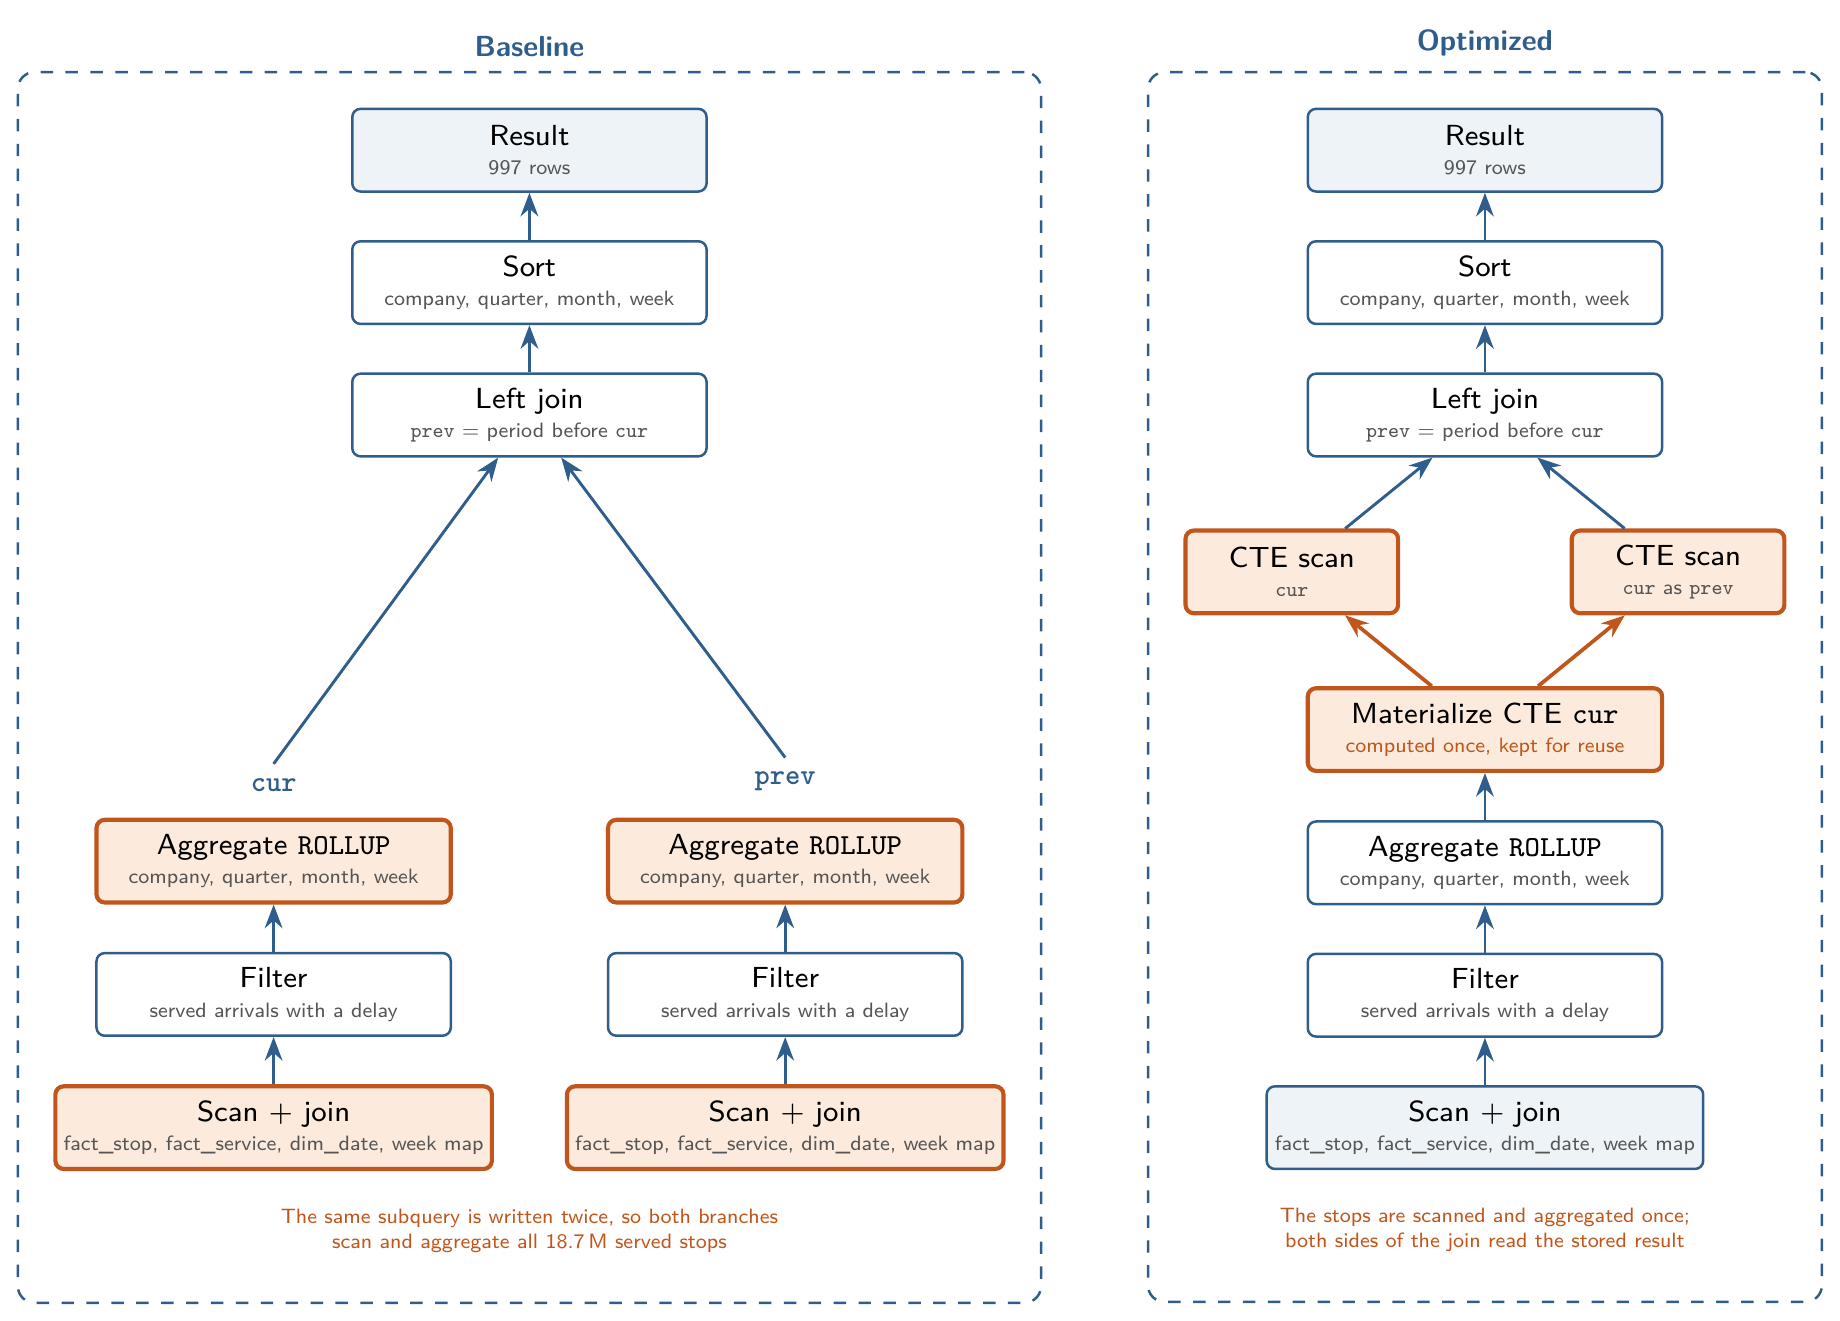
\includegraphics[width=0.8\textwidth]{figures/qpo_report1.png}
\caption{Baseline and optimized plans of Report 1. Highlighted nodes mark where the two plans differ.}
\label{fig:qpo_report1}
\end{figure*}

\begin{figure*}[t]
\centering
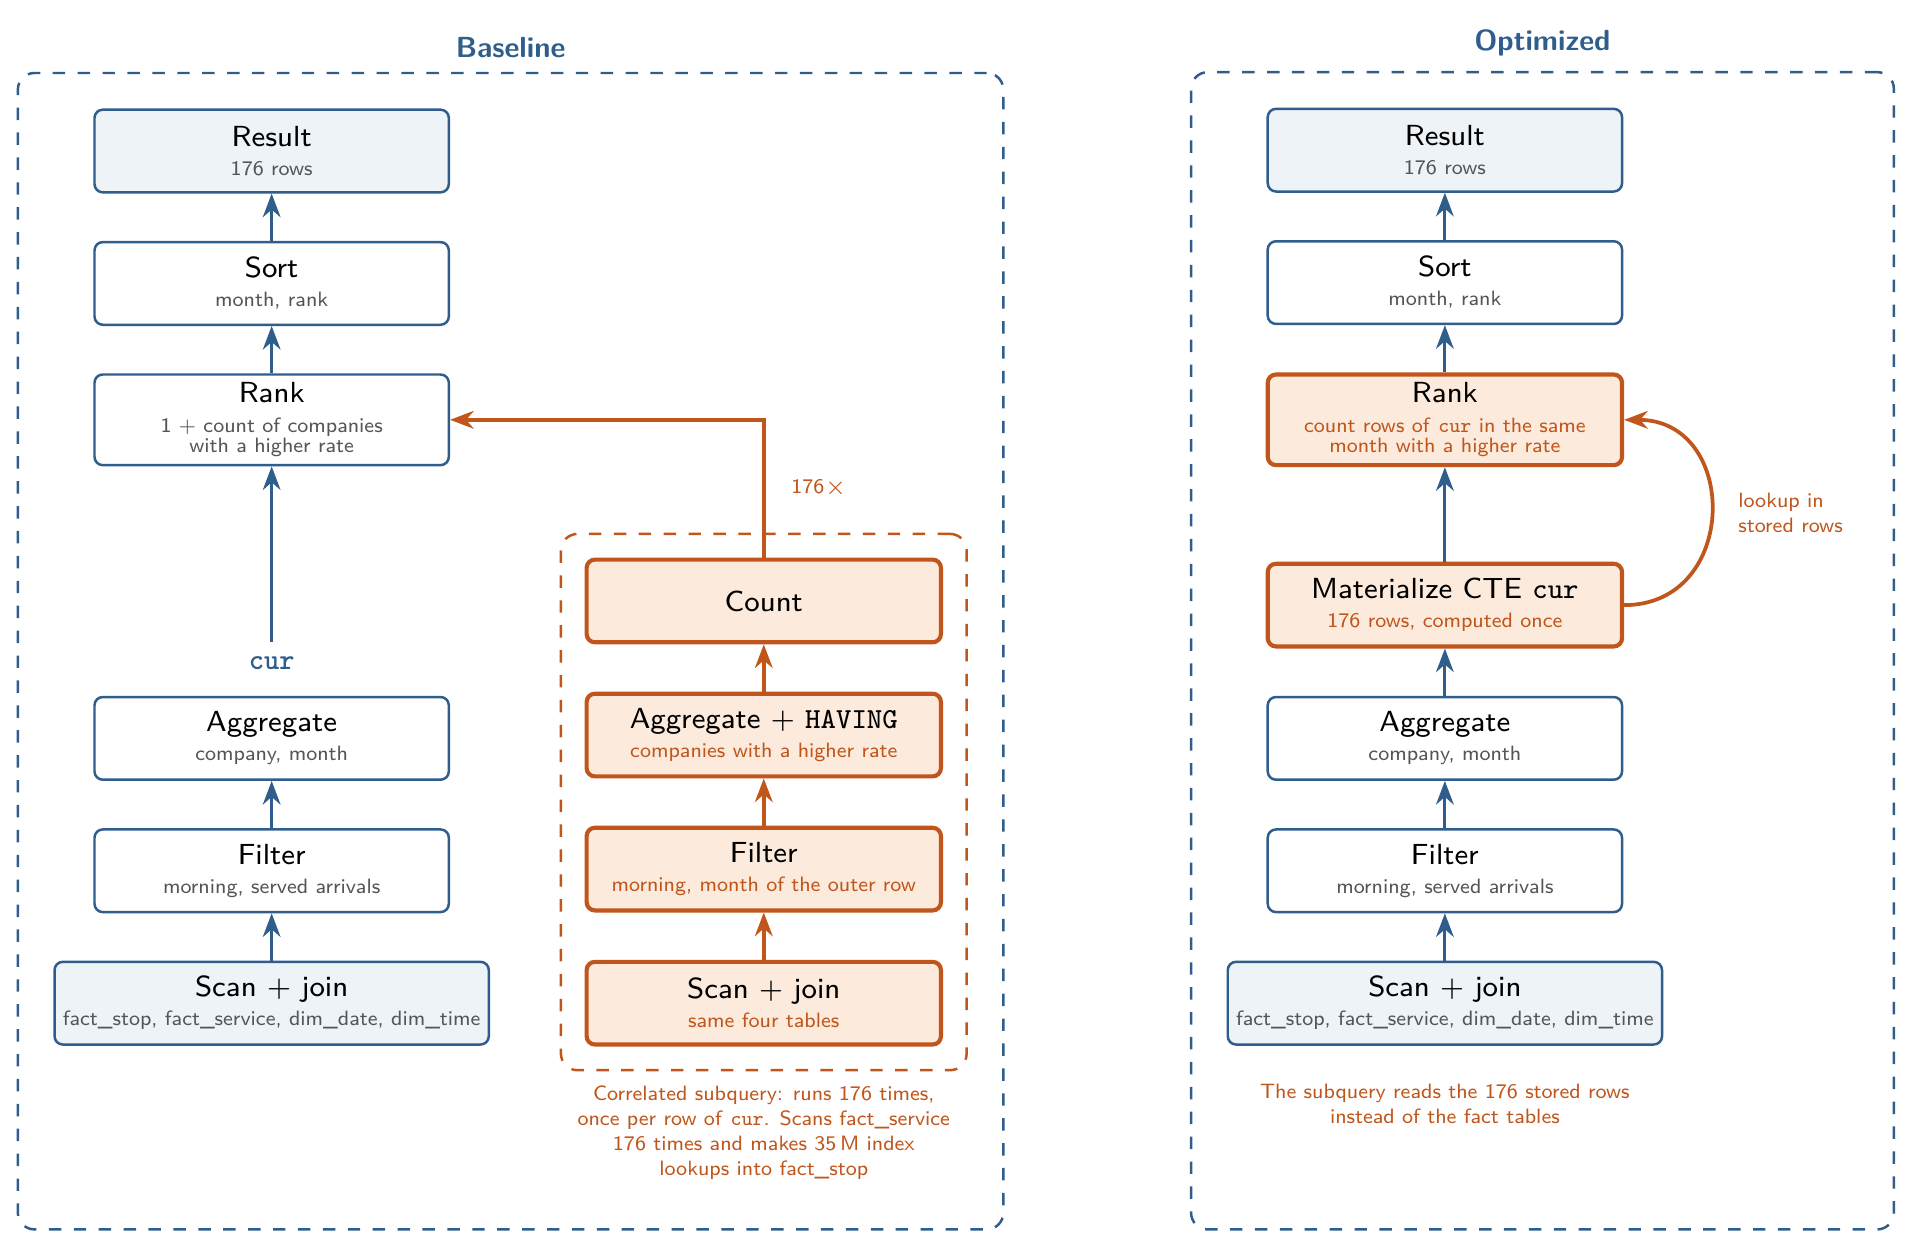
\includegraphics[width=0.8\textwidth]{figures/qpo_report2.png}
\caption{Baseline and optimized plans of Report 2. Highlighted nodes mark where the two plans differ.}
\label{fig:qpo_report2}
\end{figure*}

\begin{figure*}[t]
\centering
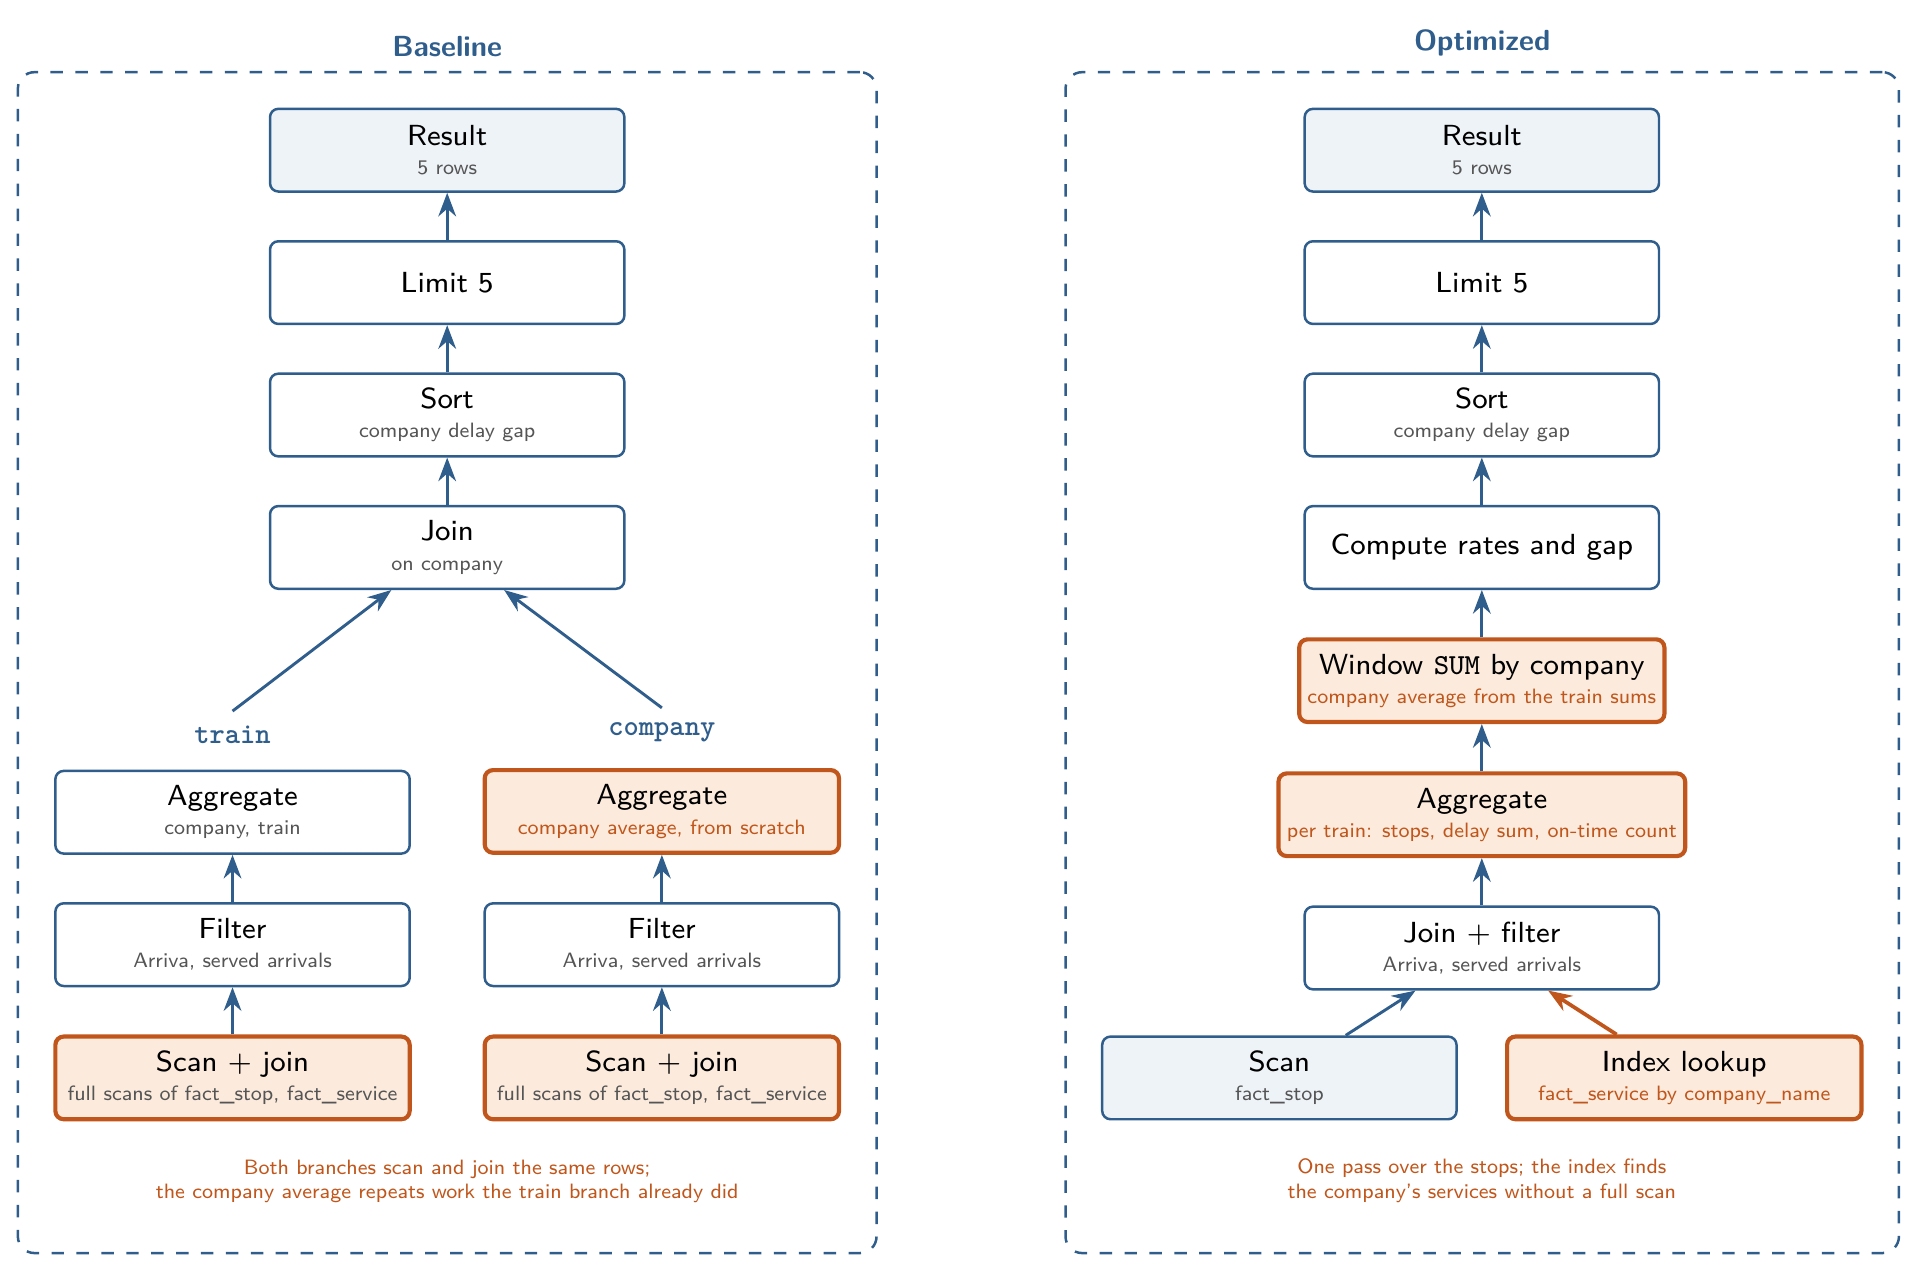
\includegraphics[width=0.8\textwidth]{figures/qpo_report3.png}
\caption{Baseline and optimized plans of Report 3. Highlighted nodes mark where the two plans differ.}
\label{fig:qpo_report3}
\end{figure*}

\begin{figure*}[t]
\centering
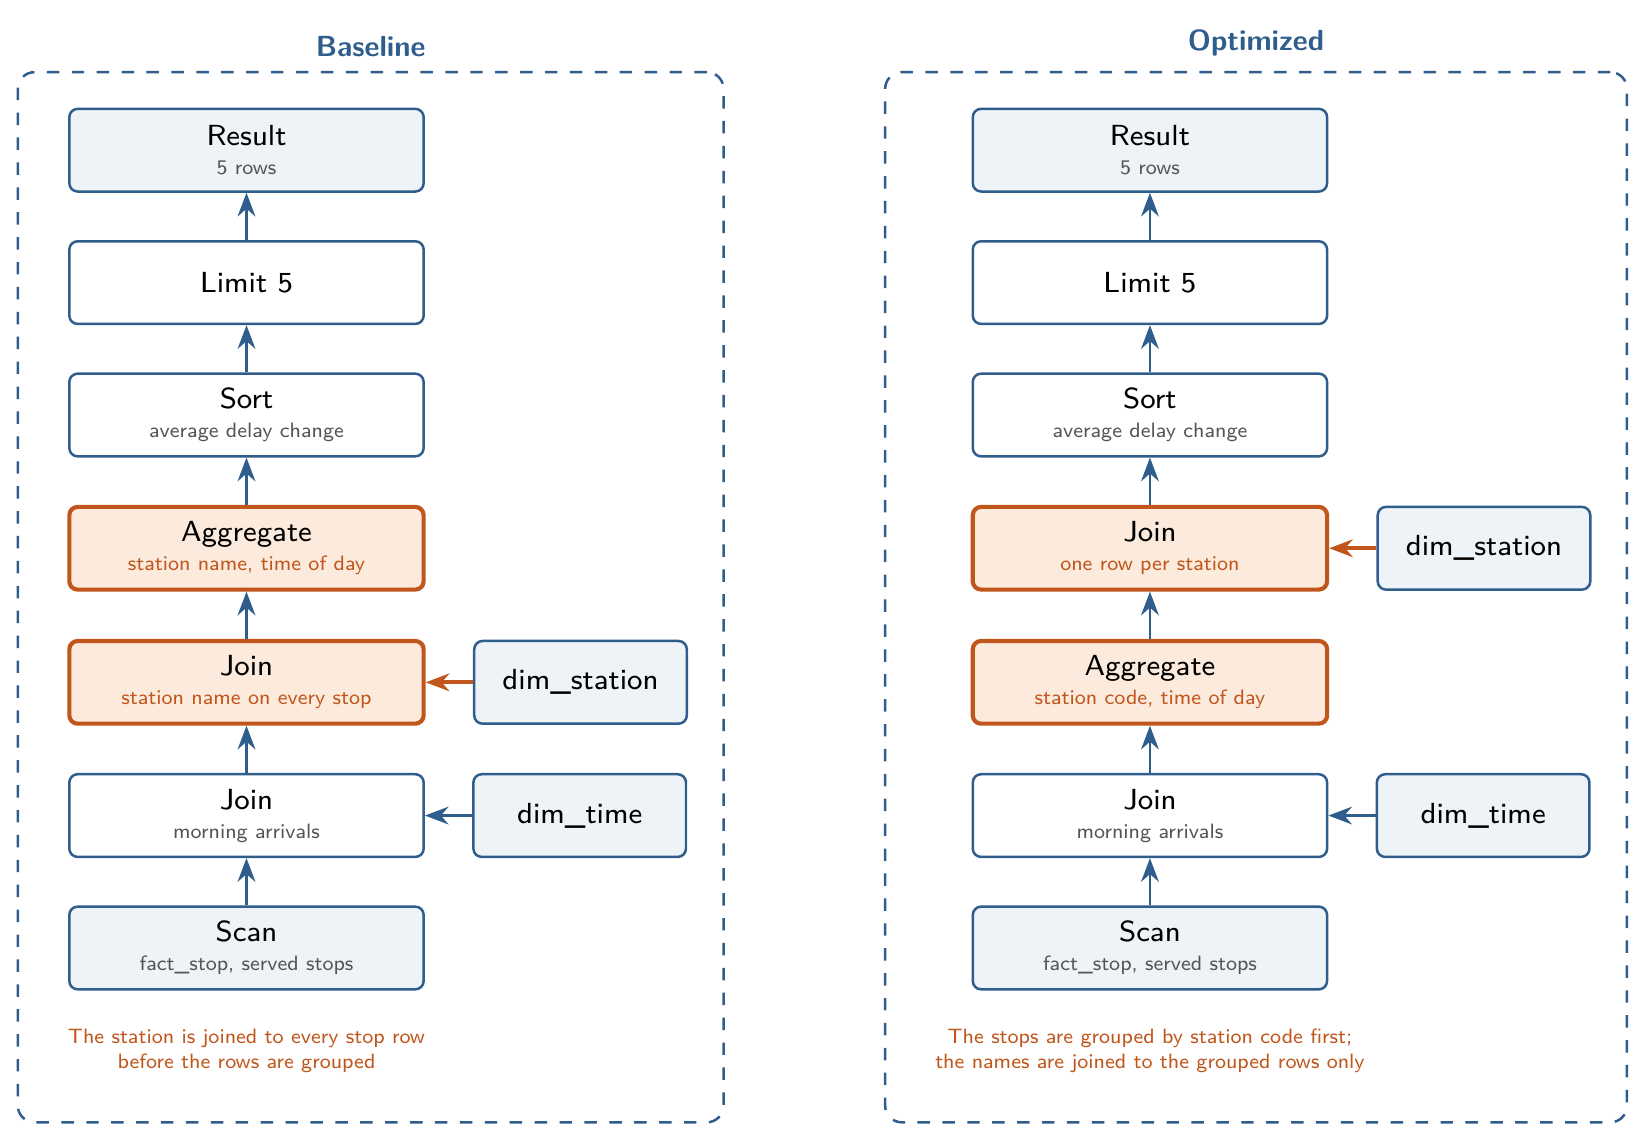
\includegraphics[width=0.8\textwidth]{figures/qpo_report4.png}
\caption{Baseline and optimized plans of Report 4. Highlighted nodes mark where the two plans differ.}
\label{fig:qpo_report4}
\end{figure*}

\subsection{Baseline Report Queries}

The baseline query for report 1 is as follows:
\begin{lstlisting}
SELECT
	cur.company_name,
	cur.quarter,
	cur.month,
	cur.week,
	cur.total_stops,
	cur.on_time_rate,
	ROUND(cur.on_time_rate - prev.on_time_rate, 2) AS rate_change

FROM (
	SELECT
		fsv.company_name,
		wm.min_quarter AS quarter,
		wm.min_month AS month,
		d.week,
		COUNT(*) AS total_stops,
		ROUND(100.0 * SUM(CASE WHEN fst.arrival_delay = 0 THEN 1 ELSE 0 END) / COUNT(*), 2) AS on_time_rate

	FROM fact_stop AS fst
	JOIN fact_service AS fsv ON fsv.rdt_id = fst.rdt_id
	JOIN dim_date AS d ON d.date_key = fsv.date_key
	JOIN (
		SELECT week, MIN(quarter) AS min_quarter, MIN(month) AS min_month
		FROM dim_date
		GROUP BY week
	) AS wm ON wm.week = d.week

	WHERE fst.cancel_status IN ('none', 'departure-only')
	AND fst.arrival_delay IS NOT NULL

	GROUP BY fsv.company_name,
	ROLLUP (wm.min_quarter, wm.min_month, d.week)
) AS cur

LEFT JOIN (
	SELECT
		fsv.company_name,
		wm.min_quarter AS quarter,
		wm.min_month AS month,
		d.week,
		ROUND(100.0 * SUM(CASE WHEN fst.arrival_delay = 0 THEN 1 ELSE 0 END) / COUNT(*), 2) AS on_time_rate

	FROM fact_stop AS fst
	JOIN fact_service AS fsv ON fsv.rdt_id = fst.rdt_id
	JOIN dim_date AS d ON d.date_key = fsv.date_key
	JOIN (
		SELECT week, MIN(quarter) AS min_quarter, MIN(month) AS min_month
		FROM dim_date
		GROUP BY week
	) AS wm ON wm.week = d.week

	WHERE fst.cancel_status IN ('none', 'departure-only')
	AND fst.arrival_delay IS NOT NULL

	GROUP BY fsv.company_name,
	ROLLUP (wm.min_quarter, wm.min_month, d.week)
) AS prev

ON prev.company_name = cur.company_name
AND (
		(cur.month IS NULL AND cur.quarter IS NOT NULL
		AND prev.month IS NULL AND prev.quarter = cur.quarter - 1)
	OR
		(cur.week IS NULL AND cur.month IS NOT NULL
		AND prev.week IS NULL AND prev.month = cur.month - 1)
	OR
		(cur.week IS NOT NULL AND prev.week = cur.week - 1)
	)

ORDER BY cur.company_name, cur.quarter, cur.month, cur.week;

\end{lstlisting}

The baseline query for report 2 is as follows:
\begin{lstlisting}
SELECT
	cur.company_name,
	cur.month,
	cur.on_time_rate,
	cur.avg_arrival_delay,
	1 + (
		SELECT COUNT(*)

		FROM (
			SELECT fsv2.company_name

			FROM fact_stop AS fst2
			JOIN fact_service AS fsv2 ON fsv2.rdt_id = fst2.rdt_id
			JOIN dim_date AS d2 ON d2.date_key = fsv2.date_key
			JOIN dim_time AS t2 ON t2.time_key = fst2.arrival_time

			WHERE fst2.cancel_status IN ('none', 'departure-only')
			AND fst2.arrival_delay IS NOT NULL
			AND t2.time_of_day = 'morning' -- THIS WHERE CLAUSE CAN CHANGE DEPENDING ON SELECTED TIME
			AND d2.month = cur.month

			GROUP BY fsv2.company_name, d2.month
			HAVING ROUND(100.0 * SUM(CASE WHEN fst2.arrival_delay = 0 THEN 1 ELSE 0 END) / COUNT(*), 2)
			       > cur.on_time_rate
		) AS better_thans
	) AS rank

FROM (
	SELECT
		fsv.company_name,
		d.month,
		ROUND(100.0 * SUM(CASE WHEN fst.arrival_delay = 0 THEN 1 ELSE 0 END) / COUNT(*), 2) AS on_time_rate,
		ROUND(AVG(fst.arrival_delay), 2) AS avg_arrival_delay

	FROM fact_stop AS fst
	JOIN fact_service AS fsv ON fsv.rdt_id = fst.rdt_id
	JOIN dim_date AS d ON d.date_key = fsv.date_key
	JOIN dim_time AS t ON t.time_key = fst.arrival_time

	WHERE fst.cancel_status IN ('none', 'departure-only')
	AND fst.arrival_delay IS NOT NULL
	AND t.time_of_day = 'morning' -- THIS WHERE CLAUSE CAN CHANGE DEPENDING ON SELECTED TIME

	GROUP BY fsv.company_name, d.month
) AS cur

ORDER BY cur.month, rank;

\end{lstlisting}


The baseline query for report 3 is as follows:
\begin{lstlisting}
SELECT
	company.company_name,
	train.train_ID,
	company.avg_delay AS avg_company_delay,
	train.on_time_rate AS train_on_time_rate,
	train.avg_delay AS avg_train_delay,
	ROUND(company.avg_delay - train.avg_delay, 2) AS company_delay_gap

FROM (
	SELECT
		fsv.company_name,
		fst.train_ID,
		ROUND(100.0 * SUM(CASE WHEN fst.arrival_delay = 0 THEN 1 ELSE 0 END) / COUNT(*), 2) AS on_time_rate,
		ROUND(AVG(fst.arrival_delay), 2) AS avg_delay
	FROM fact_stop AS fst 
	JOIN fact_service AS fsv ON fsv.rdt_id = fst.rdt_id
	WHERE fst.cancel_status IN ('none', 'departure-only')
	AND fst.arrival_delay IS NOT NULL
	AND company_name = 'Arriva' -- TO EDIT WITH SELECTED COMPANY TO CHECK DATA OF
	GROUP BY fsv.company_name, fst.train_ID
) AS train

JOIN (
	SELECT
		fsv.company_name,
		ROUND(AVG(fst.arrival_delay), 2) AS avg_delay
	FROM fact_service AS fsv
	JOIN fact_stop AS fst ON fst.rdt_id = fsv.rdt_id
	WHERE fst.cancel_status IN ('none', 'departure-only')
	AND fst.arrival_delay IS NOT NULL
	AND company_name = 'Arriva' -- TO EDIT WITH SELECTED COMPANY TO CHECK DATA OF
	GROUP BY fsv.company_name
) AS company
ON company.company_name = train.company_name

ORDER BY company_delay_gap ASC
LIMIT 5;
\end{lstlisting}


The baseline query for report 4 is as follows:
\begin{lstlisting}
SELECT
	s.station_name,
	t.time_of_day,
	ROUND(AVG(fst.departure_delay - fst.arrival_delay), 2) AS avg_delay_change,
	COUNT(*) AS total_stops
FROM fact_stop AS fst
JOIN dim_station AS s ON s.station_code = fst.station_code
JOIN dim_time    AS t ON t.time_key     = fst.arrival_time
WHERE fst.cancel_status = 'none'
AND fst.arrival_delay   IS NOT NULL
AND fst.departure_delay IS NOT NULL
AND t.time_of_day = 'morning' -- EDIT HERE TO MORNING/NOON/NIGHT BASED ON INPUT
GROUP BY s.station_name, t.time_of_day
ORDER BY avg_delay_change DESC -- EDIT HERE FROM ASC TO DESC. DESC = RECOVERY, ASC = DELAYERS
LIMIT 5;

\end{lstlisting}

\subsection{Application Wireframes}
\label{app:application_wireframes}

The following wireframes show the initial interface layout and report designs used during application planning.

\begin{figure*}[t]
\centering
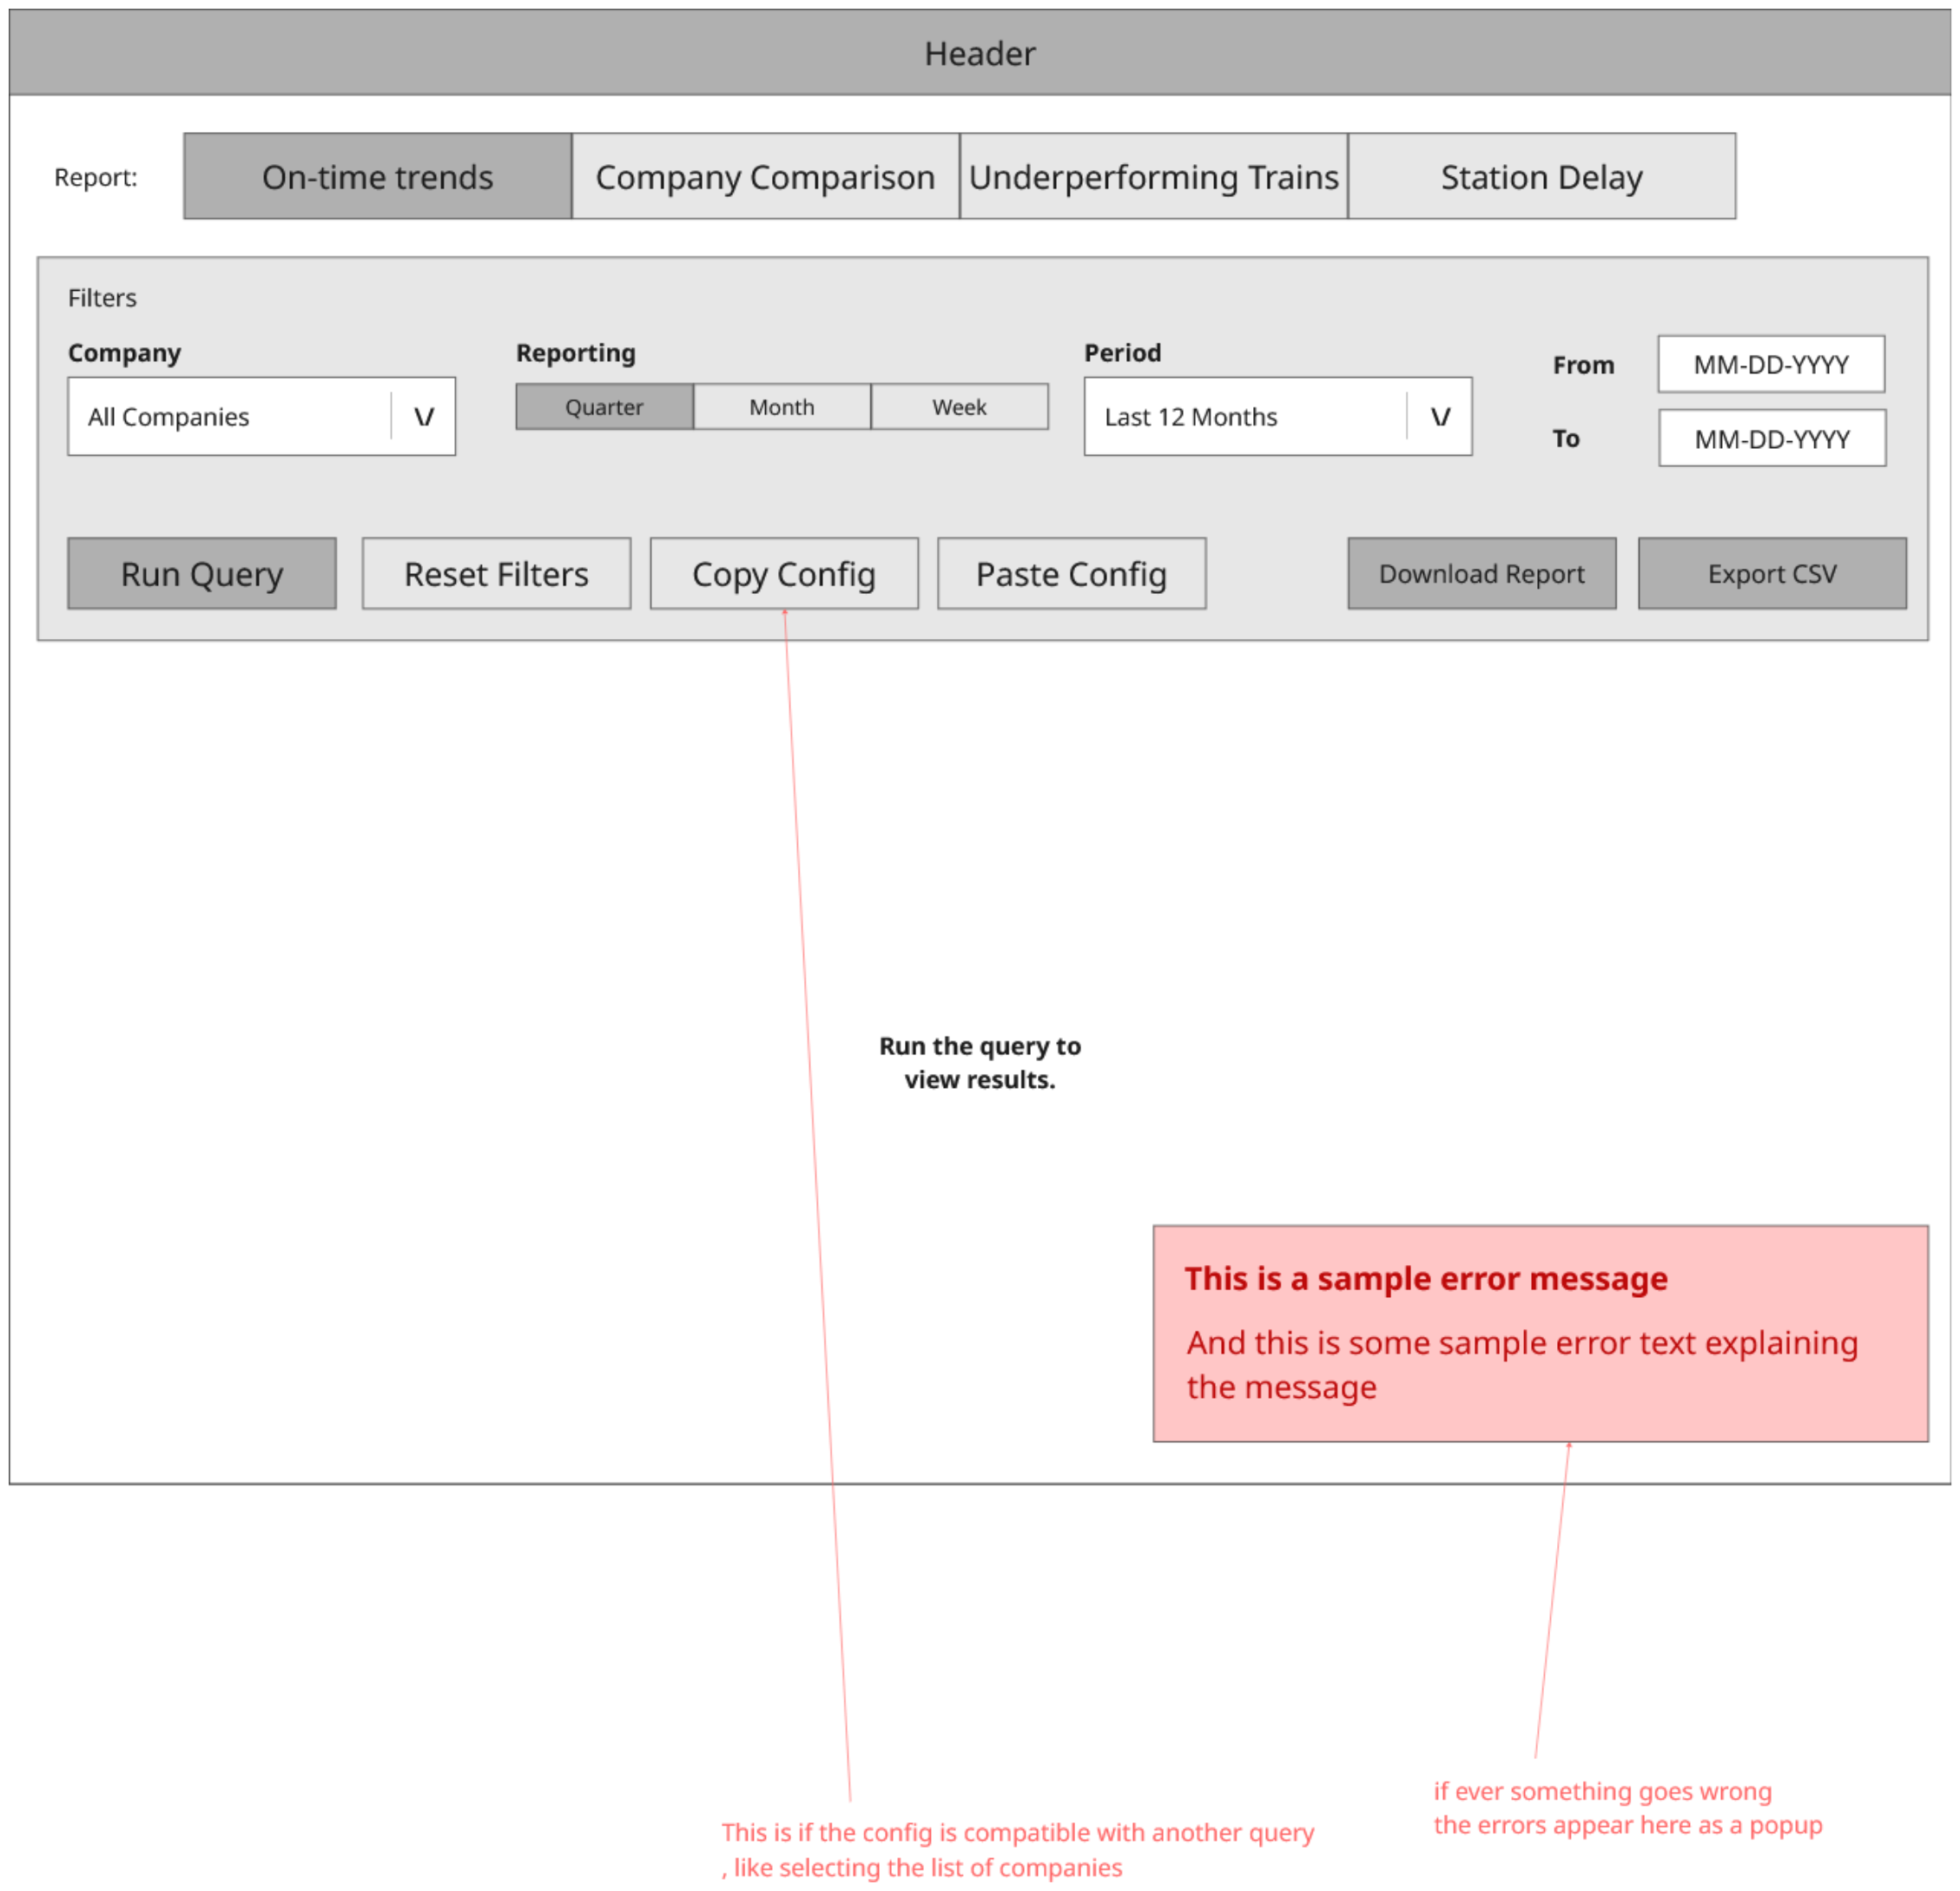
\includegraphics[width=0.9\textwidth,height=0.8\textheight,keepaspectratio]{figures/wireframe_0.png}
\caption{Initial wireframe of the shared report controls, empty results area, and error notification.}
\label{fig:wireframe_0}
\end{figure*}

\begin{figure*}[t]
\centering
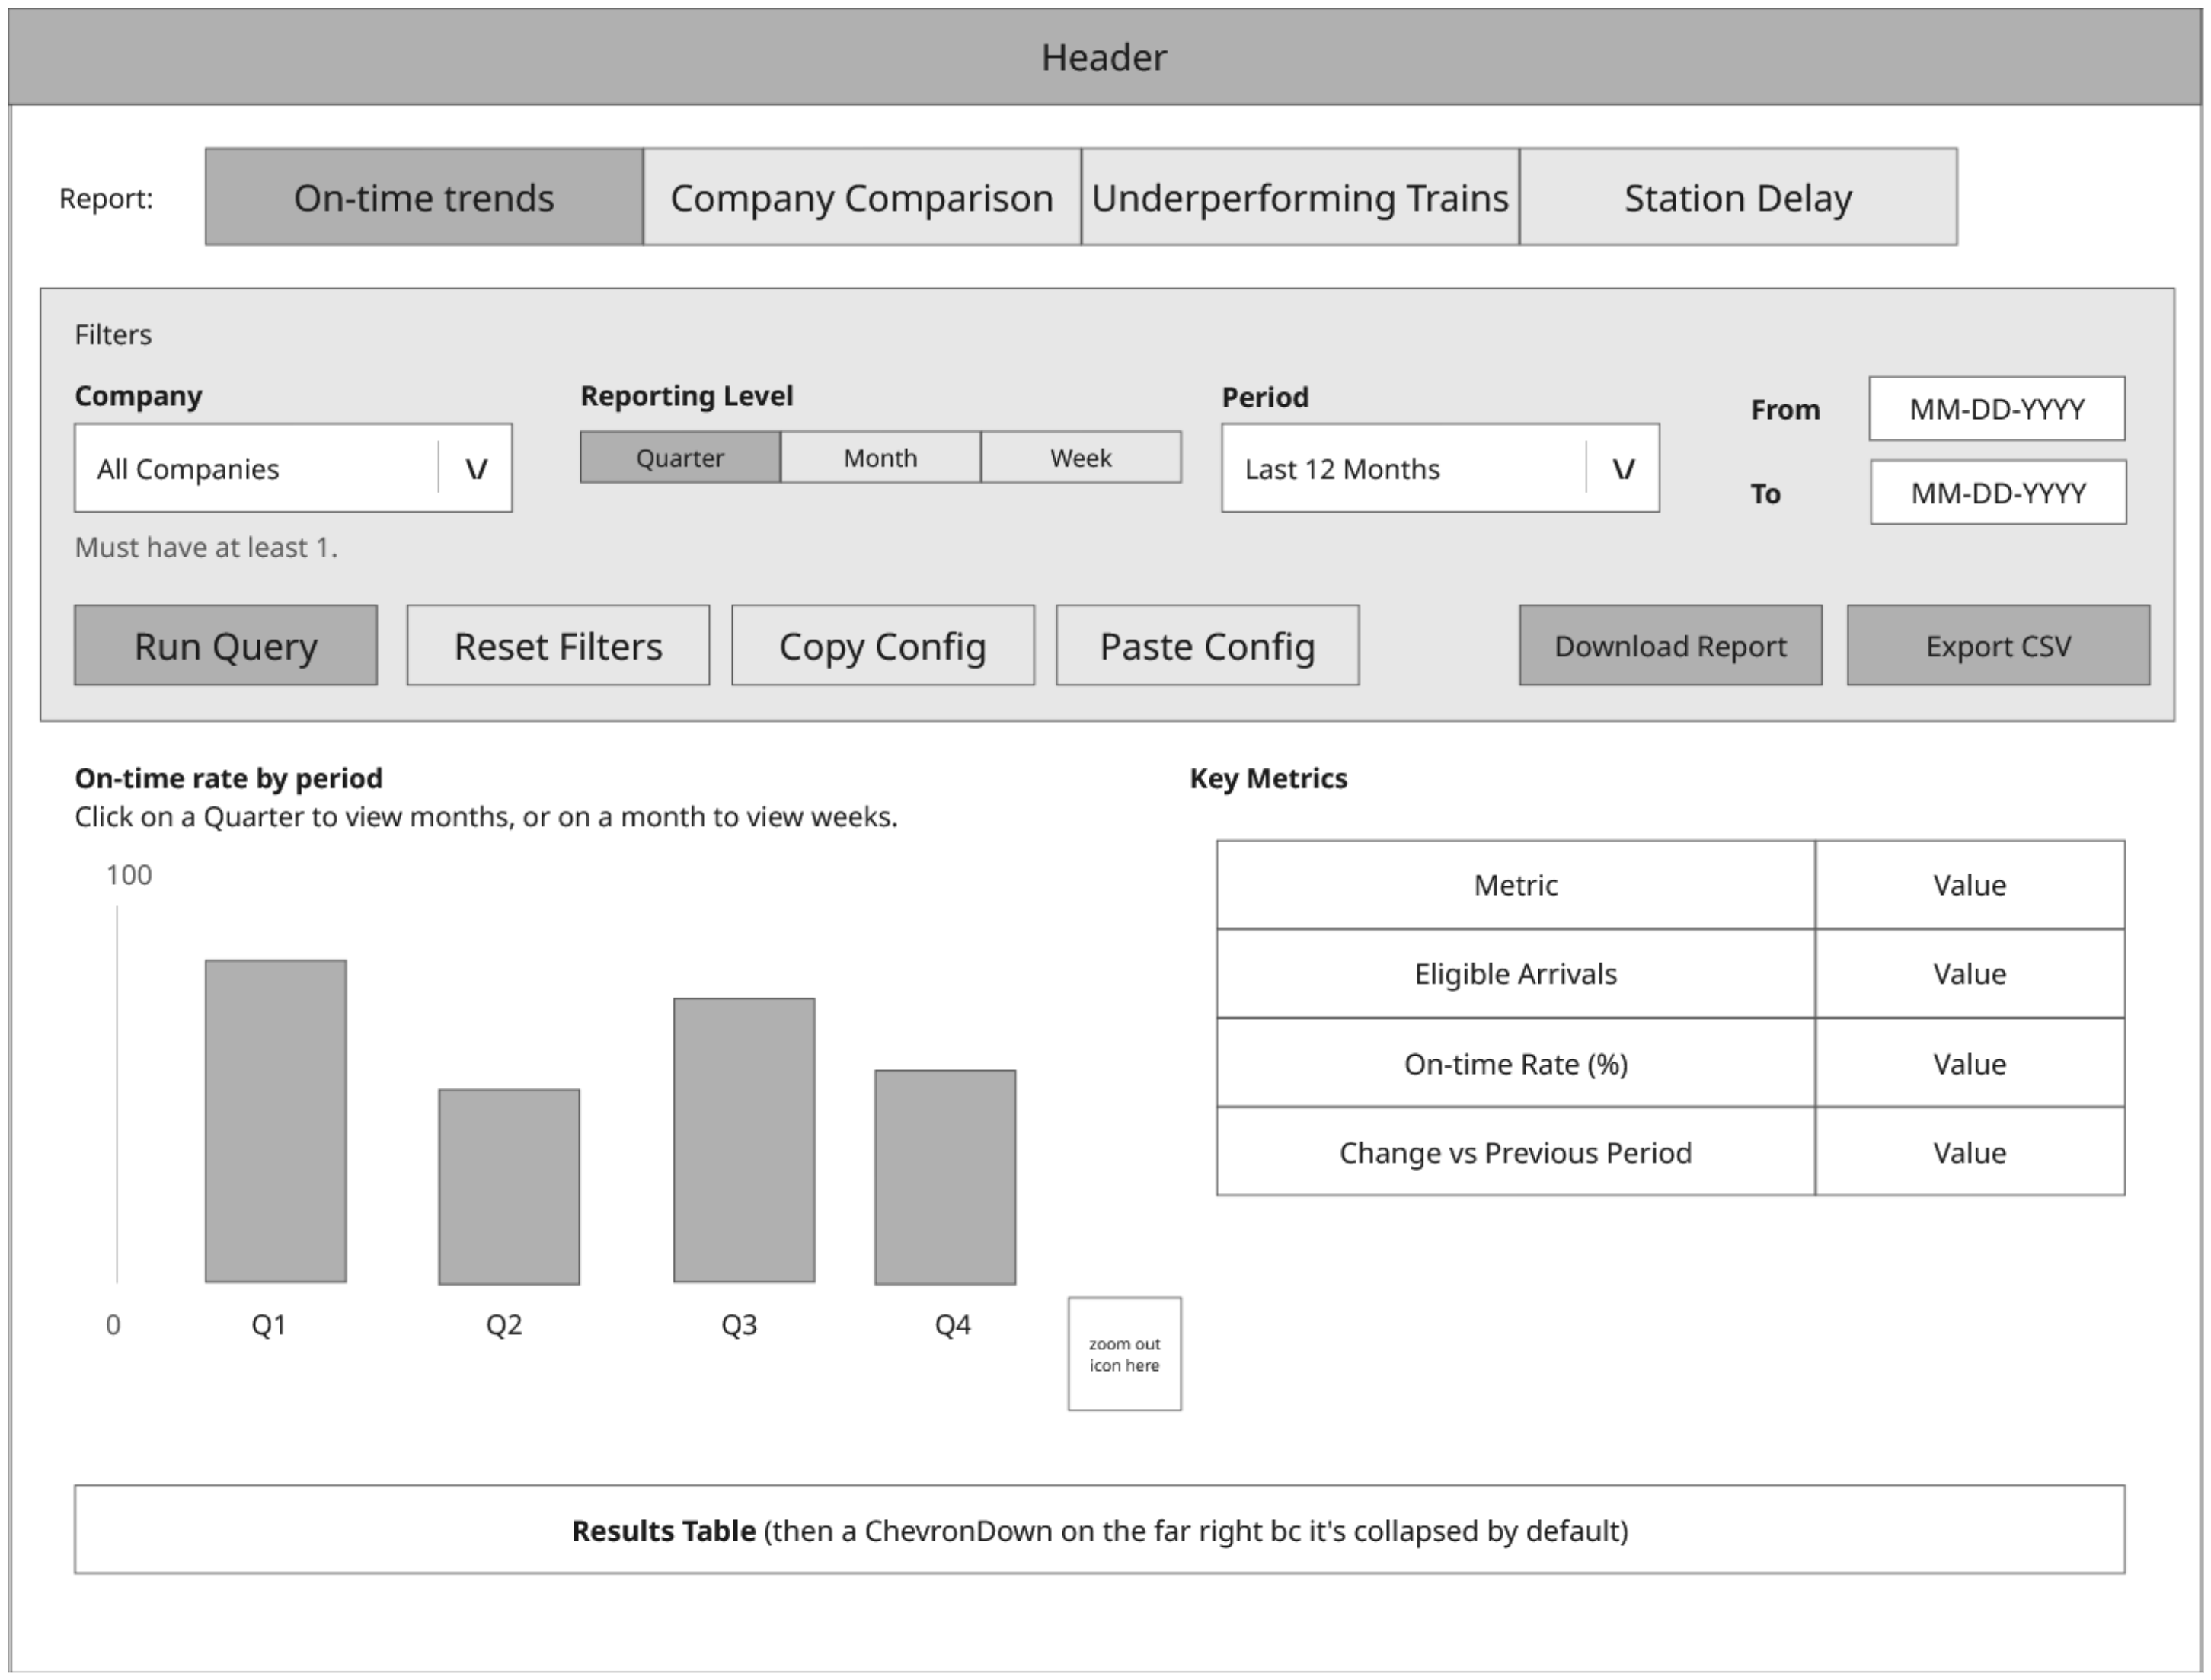
\includegraphics[width=0.9\textwidth,height=0.8\textheight,keepaspectratio]{figures/wireframe_1.png}
\caption{Initial wireframe of Report 1: On-Time Trends}
\label{fig:wireframe_1}
\end{figure*}

\begin{figure*}[t]
\centering
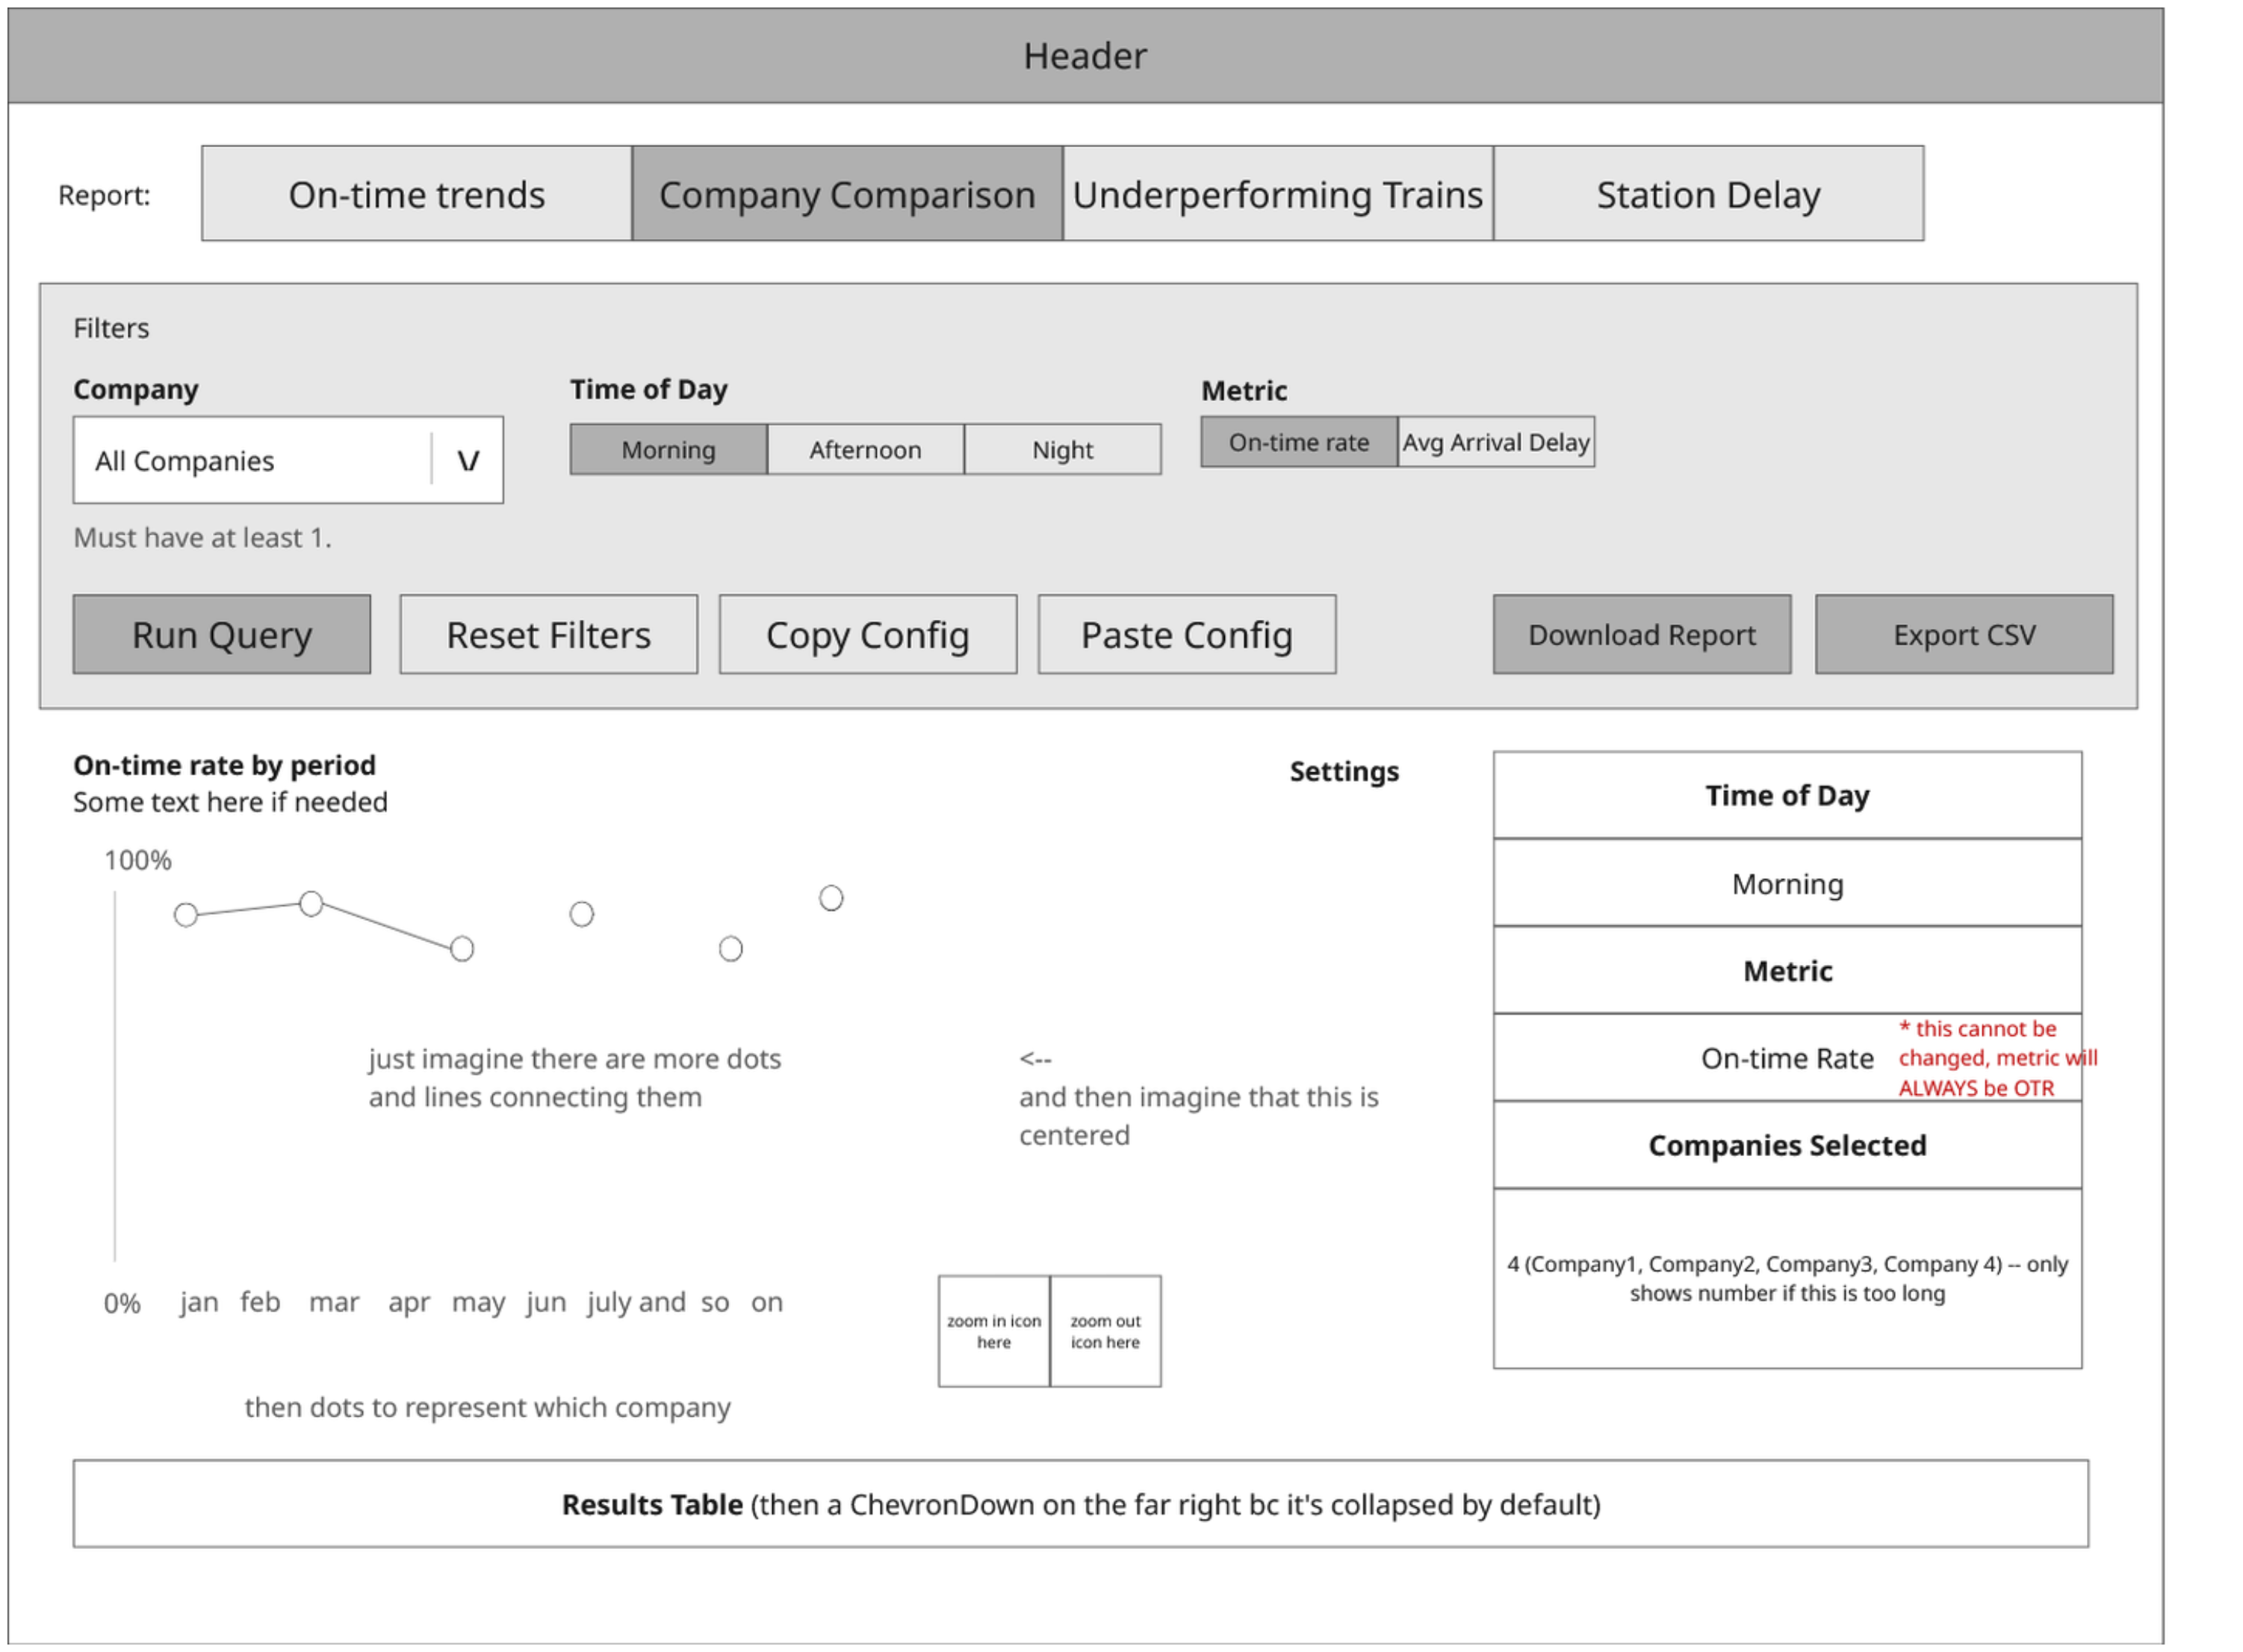
\includegraphics[width=0.9\textwidth,height=0.8\textheight,keepaspectratio]{figures/wireframe_2.png}
\caption{Initial wireframe of Report 2: Company Comparison}
\label{fig:wireframe_2}
\end{figure*}

\begin{figure*}[t]
\centering
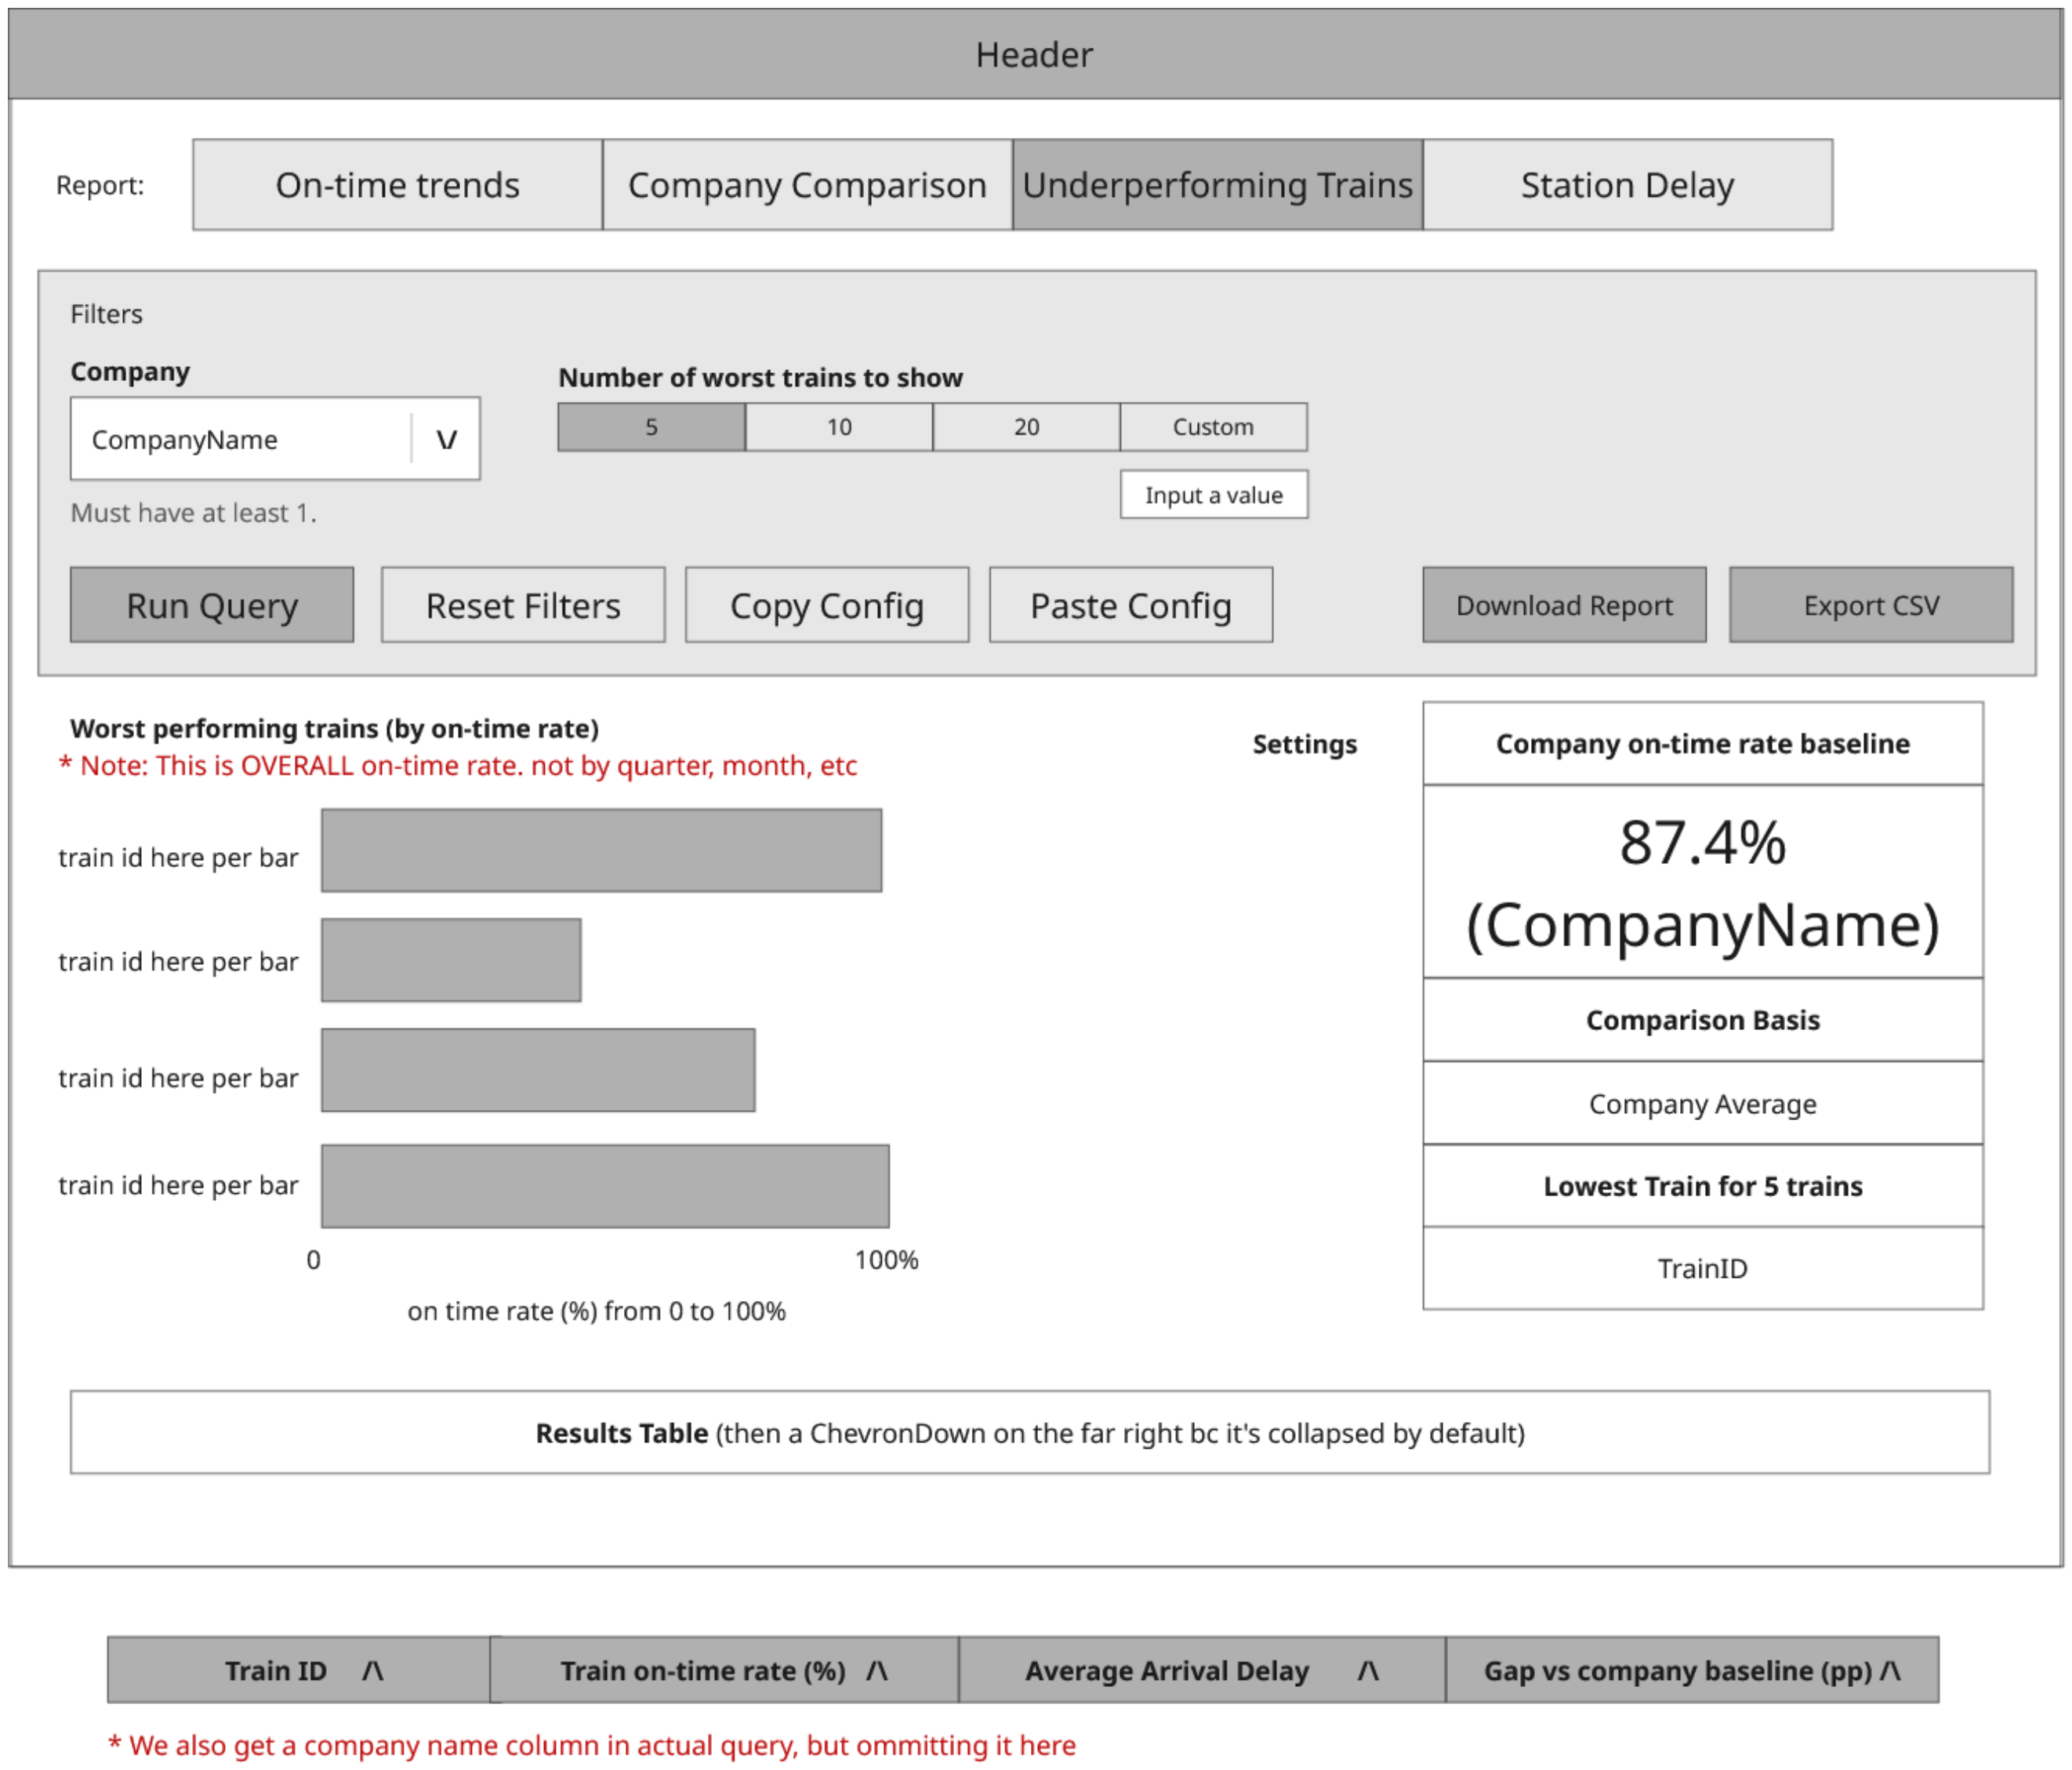
\includegraphics[width=0.9\textwidth,height=0.8\textheight,keepaspectratio]{figures/wireframe_3.png}
\caption{Initial wireframe of Report 3: Underperforming Trains}
\label{fig:wireframe_3}
\end{figure*}

\begin{figure*}[t]
\centering
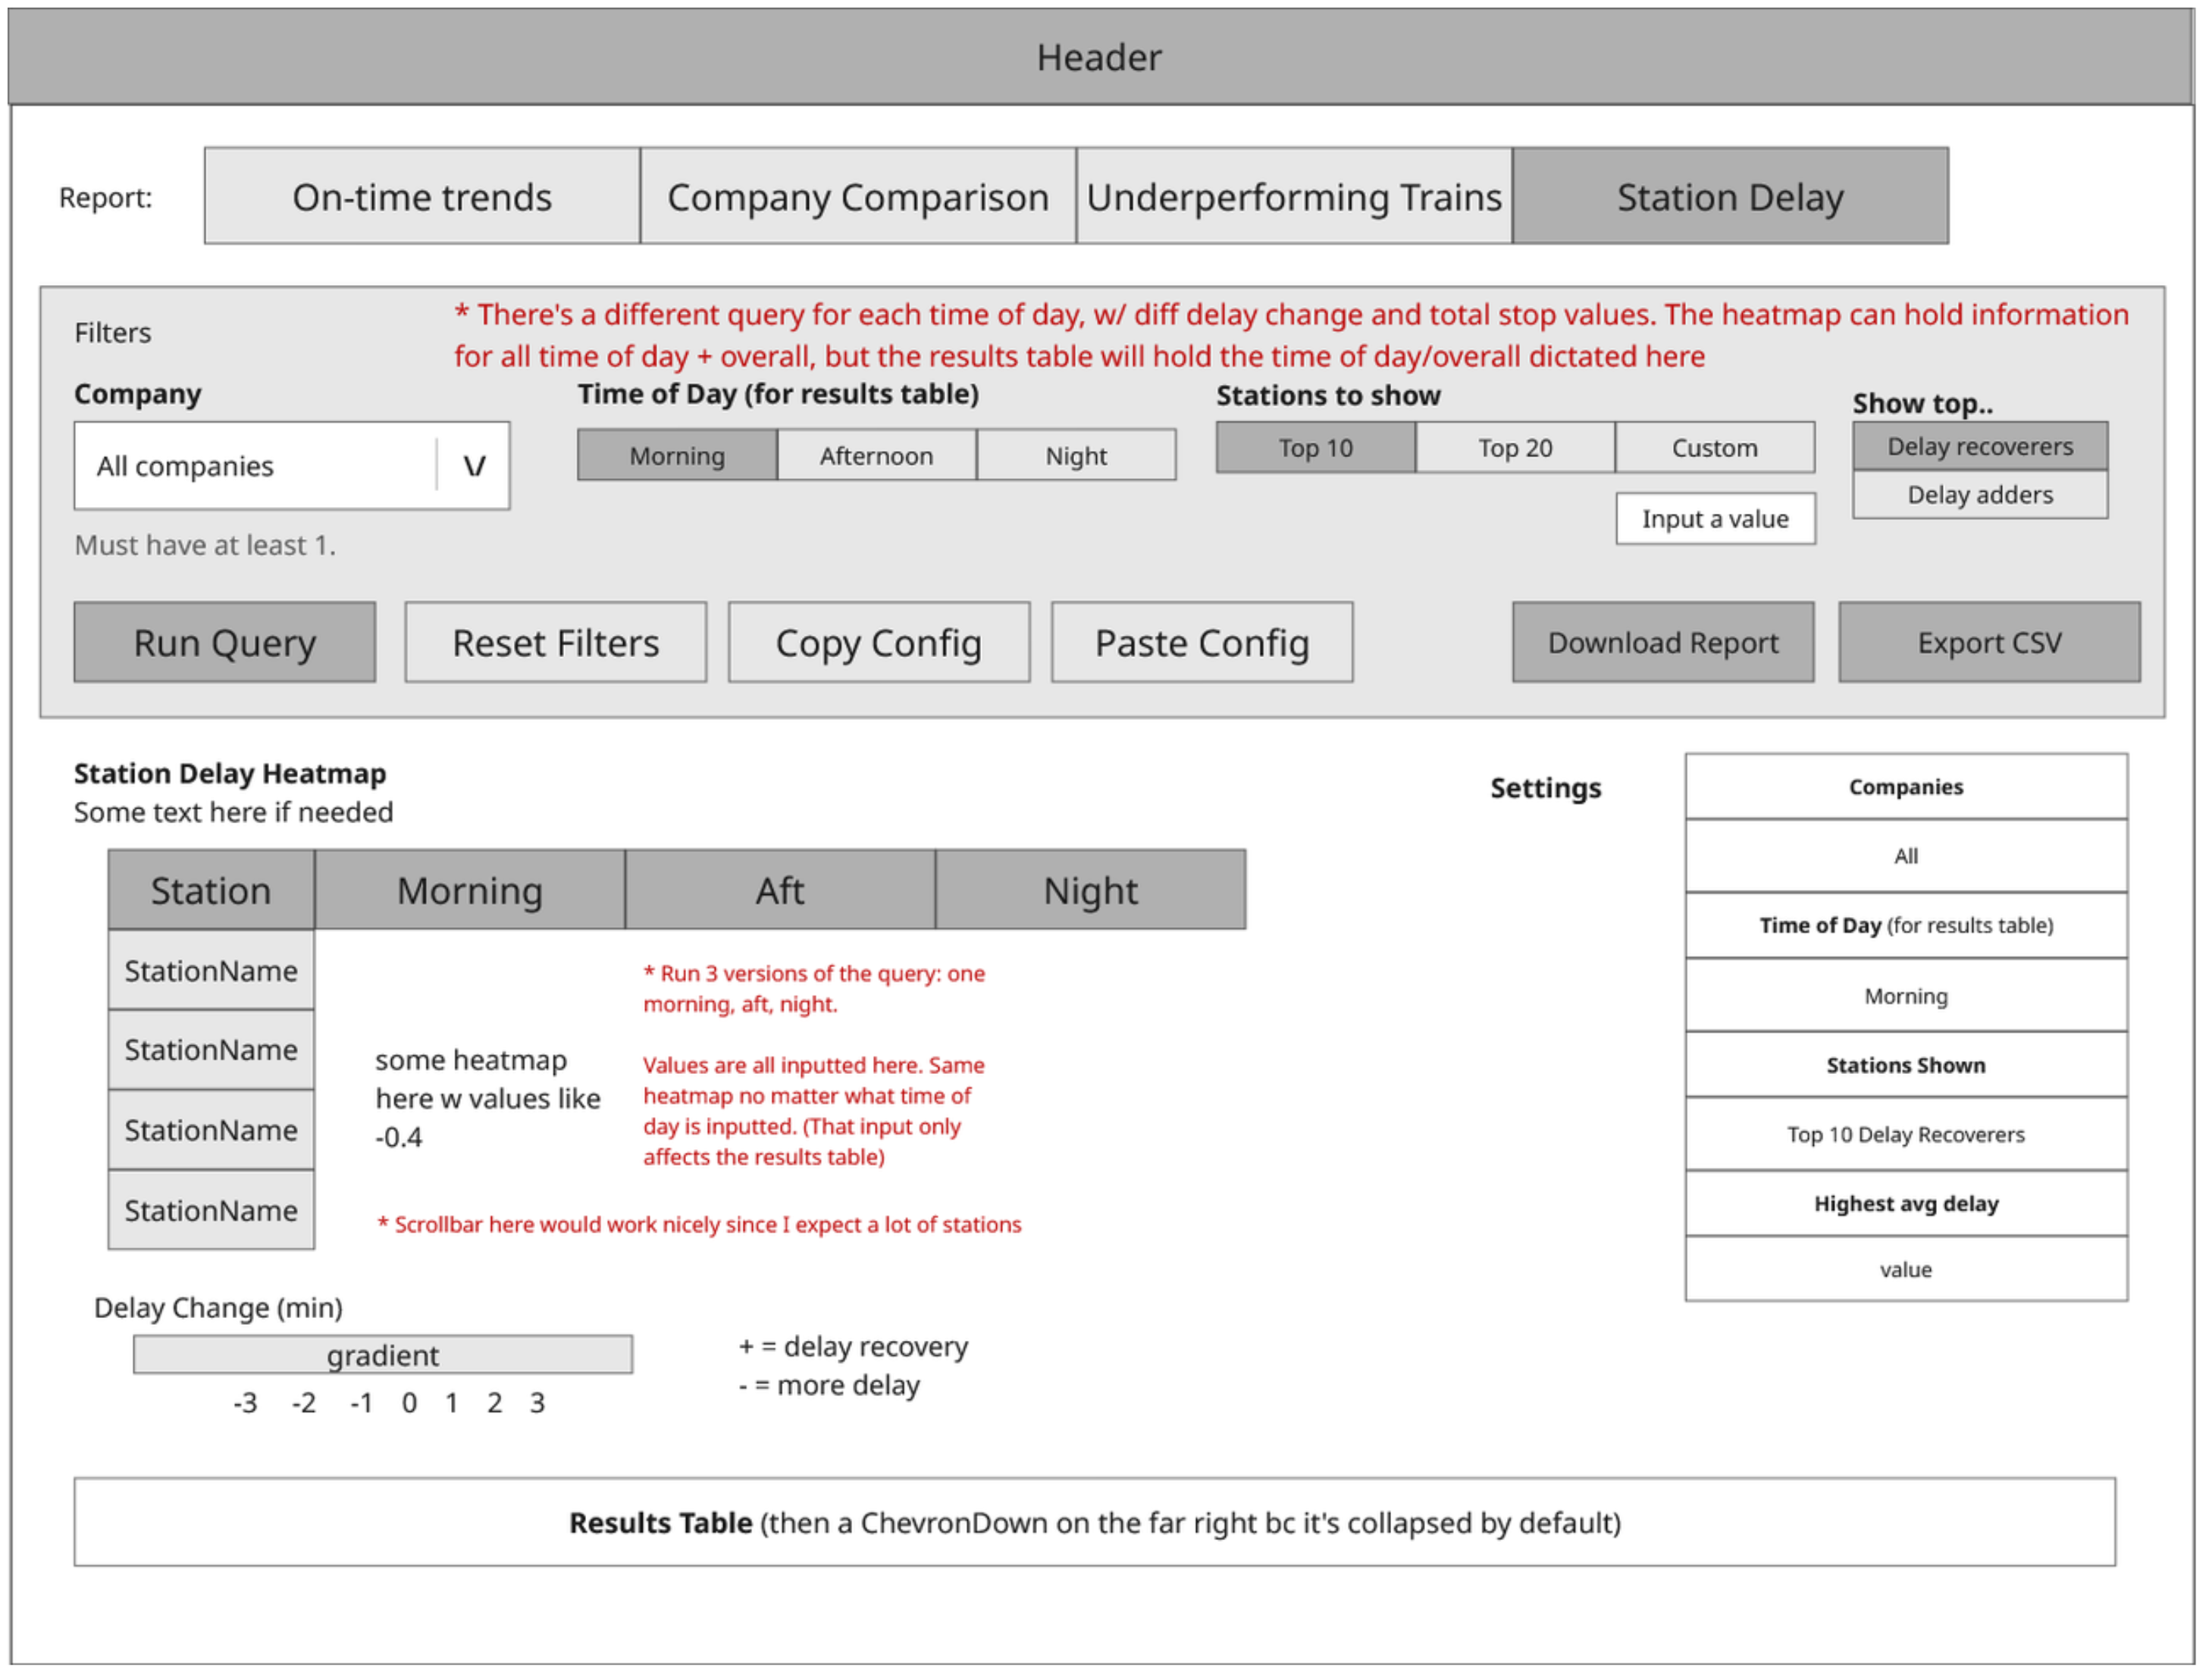
\includegraphics[width=0.9\textwidth,height=0.8\textheight,keepaspectratio]{figures/wireframe_4.png}
\caption{Initial wireframe of Report 4: Station Delay}
\label{fig:wireframe_4}
\end{figure*}
